\section{Experiments}
\label{sec:experiments}

We now test the central hypothesis of this paper: \emph{safe autoscaling
is not only a control problem, but a world-modeling problem}. A reactive
controller waits for pressure to appear; a static over-provisioning
strategy buys safety by keeping extra replicas alive; NetDream instead
learns a graph world model and uses it to imagine which scaling actions
will be safe before executing them.

First, we evaluate whether NetDream improves the cost--safety frontier
on a real Kubernetes deployment. Second, we ask whether the learned world model is accurate
enough to support short-horizon planning. Third, we ablate the two key
ingredients of NetDream: graph-structured dynamics and the safety filter.
Finally, we analyze where imagination helps most, and where Kubernetes
autoscaling remains intrinsically difficult.

\paragraph{Kubernetes testbed.}
We evaluate on Google's Online Boutique application, an 11-service
microservice system connected by 14 directed service-call dependencies.
Each service is represented by six features: CPU usage, memory usage,
queries per second, latency, error rate, and replica count. The full
state is therefore 66-dimensional. At each control step, the autoscaler
chooses a per-service action from $\{-1,0,+1\}$, corresponding to
scaling down, holding fixed, or scaling up by one replica.

We train NetDream from 48{,}000 logged transitions collected on the
Online Boutique service graph using mixed random and HPA policies. Each
transition contains the current service states, the scaling action, the
next service states, the realized reward, and whether a service-level
violation occurred. We use an 80/20 train-validation split. World-model
prediction and architecture ablations are evaluated in a calibrated
Online Boutique simulator, while closed-loop autoscaling is evaluated on
a production-grade AWS Kubernetes cluster. Metrics are collected every
5 seconds through Prometheus, workloads are generated with Locust, and
actions are applied through a custom controller that wraps the NetDream
planner.

\paragraph{Metrics and baselines.}
We measure safety by the number of service-level violations per episode.
We measure cost as total replica-steps,
\[
\mathrm{Cost}
=
0.01 \times \sum_{t=1}^{T}\sum_{s} n_s(t),
\]
where $n_s(t)$ is the number of replicas for service $s$ at time $t$.
The factor $0.01$ is a nominal per-replica-per-step rate that scales the
replica-step total into a readable range; it is not an actual cloud
price, and because every agent multiplies the same constant, relative
cost comparisons are unaffected by this choice.
Lower is better for both cost and violations.

We compare against six baselines: \emph{Random}, which samples scaling
actions uniformly; \emph{HPA}, the standard reactive Kubernetes
autoscaler tuned to a 70\% CPU target; \emph{HPA-min3} and
\emph{HPA-min5}, which add static replica floors and represent
over-provisioning as a safety strategy; \emph{PPO-500K}, a model-free
reinforcement-learning autoscaler trained for 500K simulator steps;
this configuration follows the protocol of a prior 6-algorithm RL
benchmark on the same Online Boutique testbed, which found that
flat-MLP RL trained at this budget consistently underperforms HPA
across workload classes; and
\emph{NetDream-Unsafe}, which keeps the world-model planner but removes
the safety filter. Our full method, \emph{NetDream-Safe}, uses a
3-layer GAT world model with 86K parameters, planning horizon $H=5$,
$K=64$ candidate action sequences, and safety threshold $\tau=0.5$.
All AWS Kubernetes results use three random seeds. The two most
methodologically related concurrent works, GraphPilot
\citep{chen2025graphpilot} (graph-structured actor--critic) and KARMA
\citep{karma2025} (digital-twin RL), did not have public
implementations at evaluation time; we compare against their algorithmic
paradigms (graph-predictive RL via PPO-500K and learned-dynamics
planning via NetDream itself) rather than their specific systems.

\subsection{Main Results: NetDream Improves the Cost--Safety Frontier}
\label{sec:main-results}

The main question is whether world-model planning translates into better
autoscaling on a real cluster. Table~\ref{tab:eks-summary} reports
closed-loop results on AWS Kubernetes, averaged across steady, variable,
bursty, and flash-crowd workloads.

\begin{table}[t]
\centering
\small
\caption{AWS Kubernetes results averaged across four workloads.
Lower is better for both cost and violations. Bold marks Pareto-optimal
agents.}
\label{tab:eks-summary}
\begin{tabular}{@{}lccc@{}}
\toprule
Agent & Avg.\ cost & Avg.\ violations & Cost-per-viol-reduced$^{*}$ \\
\midrule
\textbf{HPA}             & \textbf{6.8}  & 27.6 & --- \\
Random                   & 29.3 & 25.5 & $\infty$ \\
HPA-min5                 & 42.9 & 25.0 & 13.88 \\
PPO-500K                 & 35.6 & 29.7 & $\infty$ \\
NetDream-Unsafe          & 13.7 & 27.8 & $\infty$ \\
HPA-min3                 & 52.0 & 19.6 & 5.65 \\
\textbf{NetDream-Safe}   & \textbf{24.0} & \textbf{19.4} & \textbf{2.10} \\
\bottomrule
\end{tabular}
\\[2pt]
{\footnotesize
$^{*}$ Marginal cost per service-level violation reduced relative to HPA:
$\Delta\mathrm{cost}/\Delta\mathrm{violations}$.
$\infty$ means the method is both more expensive and less safe than HPA.
PPO-500K matches the training budget of a prior 6-algorithm RL benchmark
on this testbed; longer training or graph-structured policies may
improve it (see Section~\ref{sec:experiments}).
}
\end{table}

NetDream-Safe gives the best safety among all evaluated methods while
using far less cost than static over-provisioning. The Pareto frontier
has two operating points: HPA, which is cheapest, and NetDream-Safe,
which achieves the fewest violations. This is precisely the behavior we
want from a safe autoscaler: spend extra replicas only when they are
likely to prevent future violations.

Static over-provisioning also reduces violations, but it does so
inefficiently. HPA-min3 reaches a similar average violation level to
NetDream-Safe, but costs more than twice as much. In marginal terms,
NetDream-Safe reduces violations at 2.10 cost per violation avoided,
compared with 5.65 for the best static over-provisioning strategy. Thus,
NetDream is $2.7\times$ more cost-efficient at buying safety.

The result highlights the difference between \emph{more capacity} and
\emph{better capacity placement}. HPA-min3 and HPA-min5 add replicas
uniformly by raising the floor. NetDream instead uses the world model to
predict where extra replicas will matter, filters unsafe futures, and
allocates capacity selectively. This is why NetDream moves the
cost--safety frontier rather than merely sliding along it.

\begin{figure}[t]
\centering
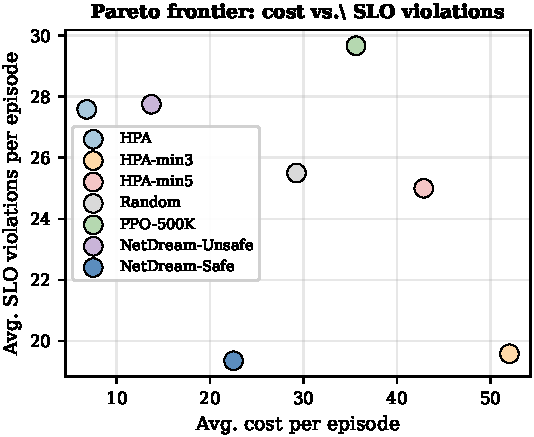
\includegraphics[width=0.55\linewidth]{figures/fig_costsafety_tradeoff.pdf}
\caption{Cost--safety Pareto frontier on AWS Kubernetes. HPA is the
lowest-cost operating point, while NetDream-Safe is the lowest-violation
operating point. NetDream-Safe provides the most cost-efficient path
toward safety.}
\label{fig:tradeoff}
\end{figure}

\subsection{World Model Analysis: Can NetDream Imagine Kubernetes Futures?}
\label{sec:prediction}

The main result depends on a necessary condition: the world model must be
accurate enough to compare short-horizon futures. We therefore evaluate
multi-step prediction error on the 11-service Kubernetes graph. The
planner does not require perfect long-term simulation; it needs a local
model that can reliably rank candidate scaling trajectories over the
next few control steps.

\begin{table}[t]
\centering
\small
\caption{Multi-step prediction accuracy on the 11-service Kubernetes
microservice graph. Lower MSE is better.}
\label{tab:prediction}
\begin{tabular}{@{}lccc@{}}
\toprule
Setting & 1-step & 5-step & 10-step \\
\midrule
Kubernetes mesh &
$2.50 \!\times\! 10^{-4}$ &
$2.09 \!\times\! 10^{-3}$ &
$4.70 \!\times\! 10^{-3}$ \\
\bottomrule
\end{tabular}
\end{table}

Table~\ref{tab:prediction} shows that NetDream maintains low error over
the planning horizon: 1-step prediction error is
$2.50\times10^{-4}$ and remains below $5\times10^{-3}$ at 10 steps. This
supports the use of short-horizon model-predictive control. NetDream is
not trying to build a perfect simulator of the entire cluster for all
future time; it only needs to imagine enough of the near future to avoid
bad scaling decisions.

The hardest feature is latency. Its prediction error is
$1.02\times10^{-2}$, much larger than the error for replica count
($5.5\times10^{-5}$). This is expected: replica count is nearly
deterministic given the action, whereas latency depends on queueing,
contention, workload shifts, and pod readiness. This observation also
foreshadows the workload-level results: NetDream is strongest when
future pressure is predictable, and weaker when violations are driven by
abrupt latency spikes.

The constraint head gives the planner an explicit safety signal. On the
Kubernetes validation set, it reaches 99.84\% F1, allowing the planner
to reject futures predicted to produce service-level violations. This is
the key difference between using a world model for passive forecasting
and using it for safe control.

\subsection{Ablation Study: Graph Structure and Safety Filtering Both Matter}
\label{sec:ablation}

We next isolate the two design choices that make NetDream work:
topology-aware world modeling and constraint-aware planning.

\paragraph{Graph structure.}
A flat neural predictor observes the same service metrics but ignores
the service-call graph. If autoscaling were simply a tabular forecasting
problem, this should be sufficient. But microservice dynamics are not
flat: load, latency, and failures propagate along service dependencies.
Figure~\ref{fig:ablation} compares GAT, GCN, GraphSAGE, and an MLP
without graph structure.

\begin{figure}[t]
\centering
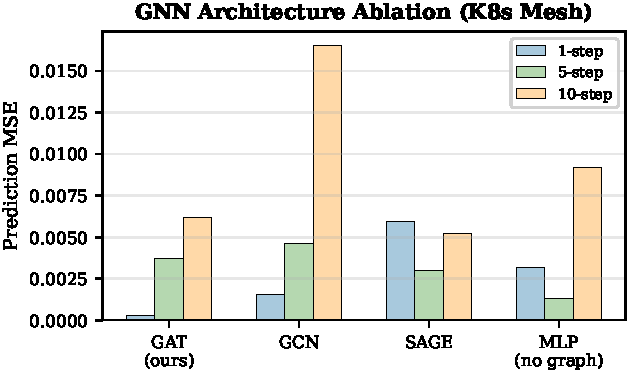
\includegraphics[width=0.48\textwidth]{figures/fig_gnn_ablation.pdf}
\caption{Architecture ablation on Kubernetes dynamics prediction.
Removing graph structure increases 1-step prediction error by
$11\times$, showing that graph structure is required for reliable
multi-step prediction.}
\label{fig:ablation}
\end{figure}

Removing graph structure increases one-step prediction error by
$11\times$. This is not simply a capacity effect: a GCN with the same
parameter count as the GAT still substantially outperforms the MLP. The
service-call topology itself provides the inductive bias needed to model
how pressure propagates through the system. Among graph models, GAT
achieves the best one-step accuracy, suggesting that attention is useful
for heterogeneous dependencies: not all service edges carry equal
influence.

\paragraph{Safety filtering.}
The second ablation removes the safety filter while keeping the learned
world model and planner. NetDream-Unsafe is cheaper than NetDream-Safe,
but it does not improve violations over HPA. This shows that prediction
alone is not enough. A world model can propose high-reward futures that
still carry unacceptable violation risk; the safety filter is what turns
imagination into safe imagination.

Together, these ablations clarify the mechanism behind NetDream's gains.
The graph world model provides useful futures, and the safety filter
decides which futures are acceptable. Removing either component weakens
the controller: without the graph, the imagined dynamics are inaccurate;
without the filter, the planner does not reliably avoid unsafe actions.

\subsection{Workload Analysis: When Does Imagination Help Most?}
\label{sec:workload-analysis}

The aggregate result hides an important pattern: NetDream helps most
when the workload changes enough that reactive control lags, but not so
abruptly that pod startup time dominates the episode.

\begin{figure}[t]
\centering
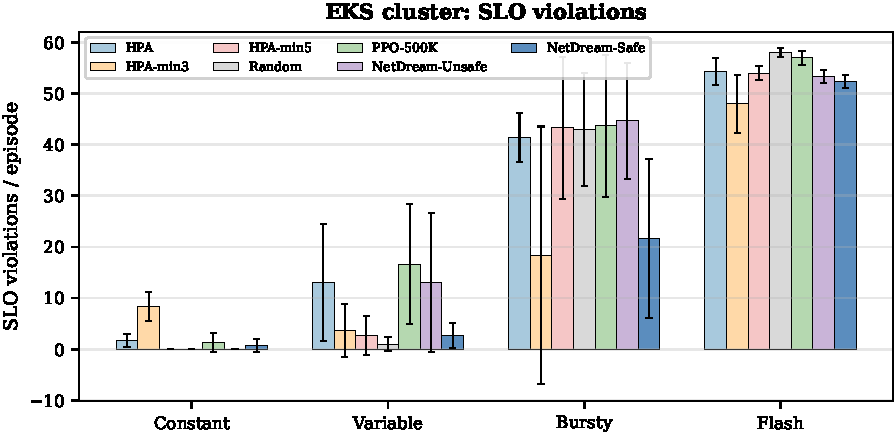
\includegraphics[width=0.95\linewidth]{figures/fig_planning_violations.pdf}
\caption{Service-level violations per episode on AWS Kubernetes by
workload. NetDream-Safe achieves about $5\times$ fewer violations than
HPA on variable traffic.}
\label{fig:planning}
\end{figure}

\begin{figure}[t]
\centering
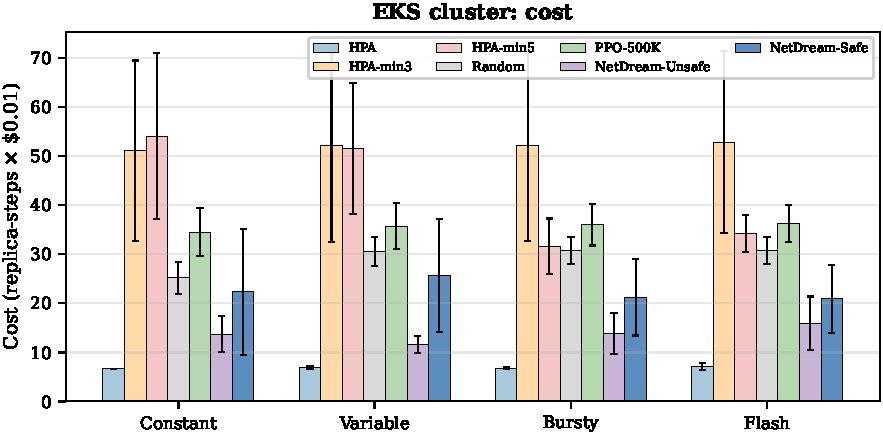
\includegraphics[width=0.95\linewidth]{figures/fig_cost_comparison.pdf}
\caption{Replica-step cost on AWS Kubernetes by workload. Static
over-provisioning reduces violations only by paying substantially higher
replica cost.}
\label{fig:cost}
\end{figure}

The clearest win is variable traffic. NetDream-Safe reduces violations
from 13.0 to 2.7 compared with HPA, a nearly $5\times$ reduction, while
using about half the cost of HPA-min5, the strongest static floor
baseline with comparable safety on this workload. This is the ideal
regime for world-model planning: the system is changing, so reactive
thresholds lag, but the future is still predictable enough for the model
to allocate replicas before violations occur.

Steady traffic is less dramatic because HPA is already strong when the
system is stable. In this regime, there is less future uncertainty to
exploit, so the advantage of imagination is smaller. Bursty and
flash-crowd traffic are difficult for a different reason: latency can
spike faster than new replicas become ready. This exposes a physical
limit of pod-level autoscaling. No planner can fully prevent violations
when capacity is needed before Kubernetes can start it.

This analysis sharpens the interpretation of NetDream. Its advantage is
not that it magically eliminates all violations. Its advantage is that
it spends replica budget where prediction is actionable. When future
pressure is visible through the service graph, NetDream can act before
the threshold is crossed. When the bottleneck is pod startup latency
under abrupt flash traffic, better planning must be paired with online
adaptation or node-level capacity planning.

Overall, the experiments support the paper's central claim: the path to
safe and efficient Kubernetes autoscaling is not static
over-provisioning or model-free reaction, but planning over a learned
graph model on this benchmark.
By learning a graph world model and planning through it, NetDream can
predict which futures are unsafe, reject them before execution, and move
the system to a better cost--safety frontier.